\section{API Documentation}
Le API fornite dall’applicazione JGuesser sono
state documentate utilizzando Swagger UI Express. In questo
modo la documentazione relativa alle API è direttamente disponibile a chiunque le voglia utilizzare per altri progetti. È possibile accedere alla documentazione tramite il seguente link in locale: \href{localhost:8080/api-docs/}{localhost:8080/api-docs/}, oppure accedendo all'URI: /api-docs/ in remoto (con dominio del server). Nel nostro caso il link è il seguente: \href{https://JGuesser-BackEnd-Unitn.up.railway.app/api-docs/}{https://JGuesser-BackEnd-Unitn.up.railway.app/api-docs/}.

\begin{figure}[!h]
\centering
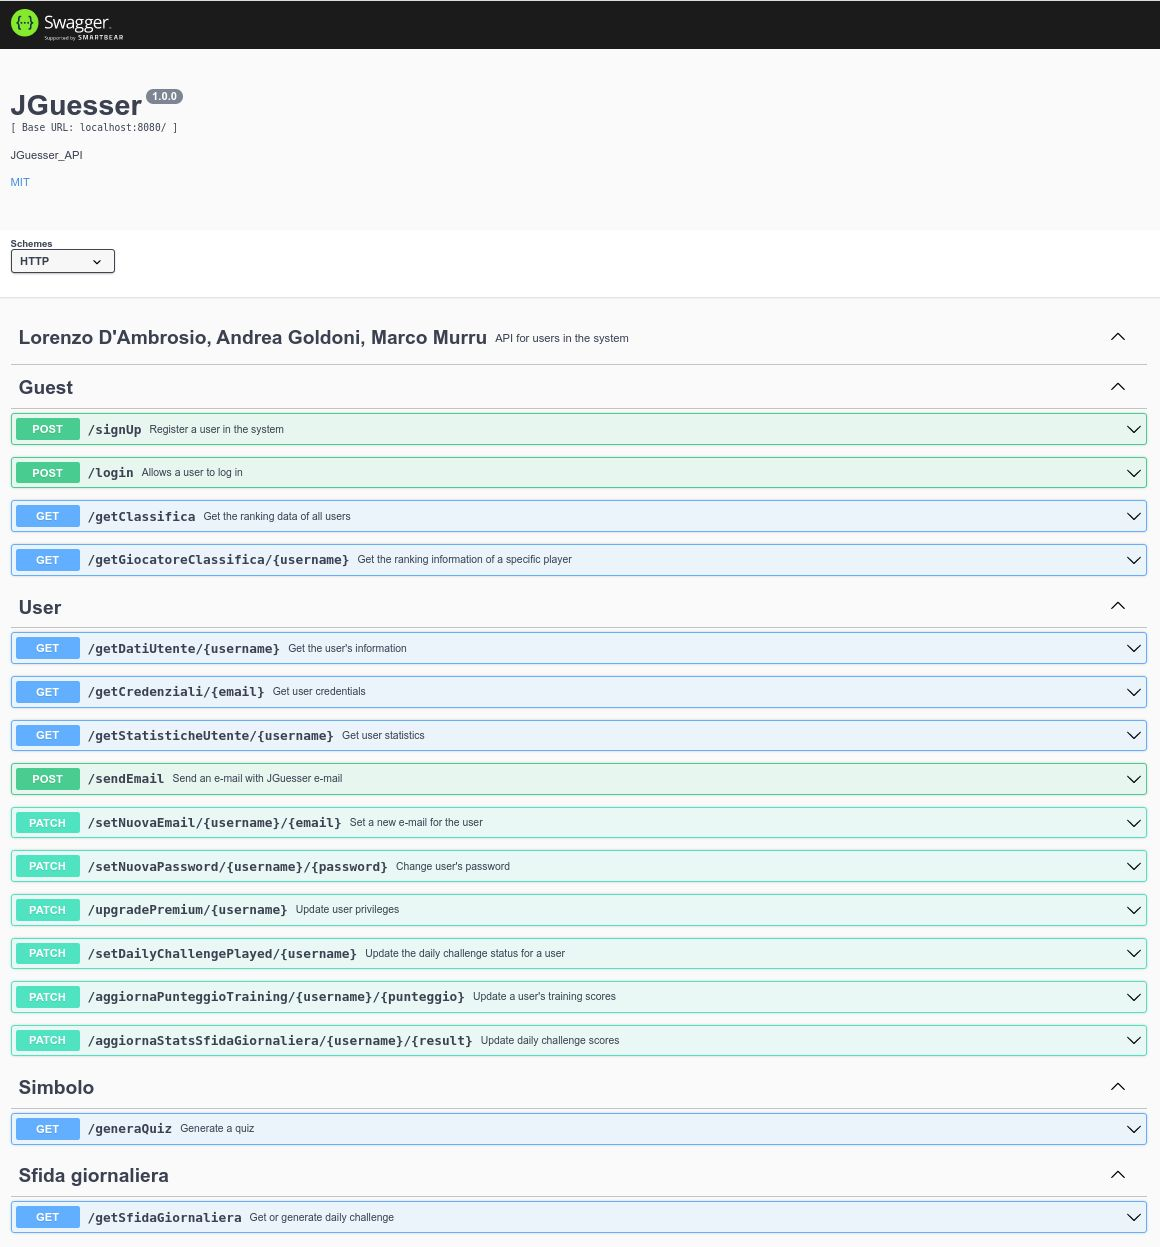
\includegraphics[scale=0.5]{images/swagger_api_documentation.jpg}
\caption{Documentazione delle API di JGuesser}
\label{fig:swagger_api_documentation}
\end{figure}
\noindent